\section{IPFS} \label{section:2-7-ipfs}

\logo{chapter-2/2.7.ipfs-logo}{IPFS logo}

Το IPFS (InterPlanetary File System) είναι \textit{ένα P2P πρωτόκολλο υπερμέσων, σχεδιασμένο για να διατηρήσει και να αυξήσει τη γνώση της ανθρωπότητας κάνοντας το διαδίκτυο αναβαθμίσιμο, ανθεκτικό και πιο ανοιχτό}.\cite{2.7-ipfs}
Πρακτικά πρόκειται για ένα κατανεμημένο σύστημα για αποθήκευση και πρόσβαση σε αρχεία, ιστότοπους, εφαρμογές και δεδομένα. Το περιεχόμενο είναι προσβάσιμο μέσω ενός δικτύου ομότιμων κόμβων που βρίσκονται οπουδήποτε στον κόσμο, οι οποίοι ενδέχεται να να αποθηκεύουν πληροφορία, να τη μεταφέρουν (relay nodes) ή και τα δύο.\cite{2.7-ipfs-docs}

Ο τρόπος λειτουργίας του IPFS βασίζεται στα εξής:

\begin{itemize}
	\item \textbf{Μοναδική ταυτοποίηση μέσω διευθυνσιοδότησης περιεχομένου (content addressing)}. Το περιεχόμενο δεν προσδιορίζεται από την τοποθεσία του (π.χ. https://...), αλλά από το τι περιλαμβάνει. Κάθε κομμάτι περιεχομένου έχει ένα μοναδικό αναγνωριστικό (Content ID ή CID), το οποίο είναι το hash του σε μορφή multihash (\url{https://multiformats.io/multihash/}).
	\item \textbf{Σύνδεση περιεχομένου μέσω κατευθυνόμενων άκυκλων γράφων (Directed Acyclic Graphs ή DAGs)}. Το IPFS αξιοποιεί DAGs (και συγκεκριμένα Merkle DAGs), μίας δομής δεδομένων της οποίας κάθε κόμβος έχει ως μοναδικό αναγνωριστικό το hash του περιεχομένου του (το CID).

	\begin{enumitemcenteredfigure}
		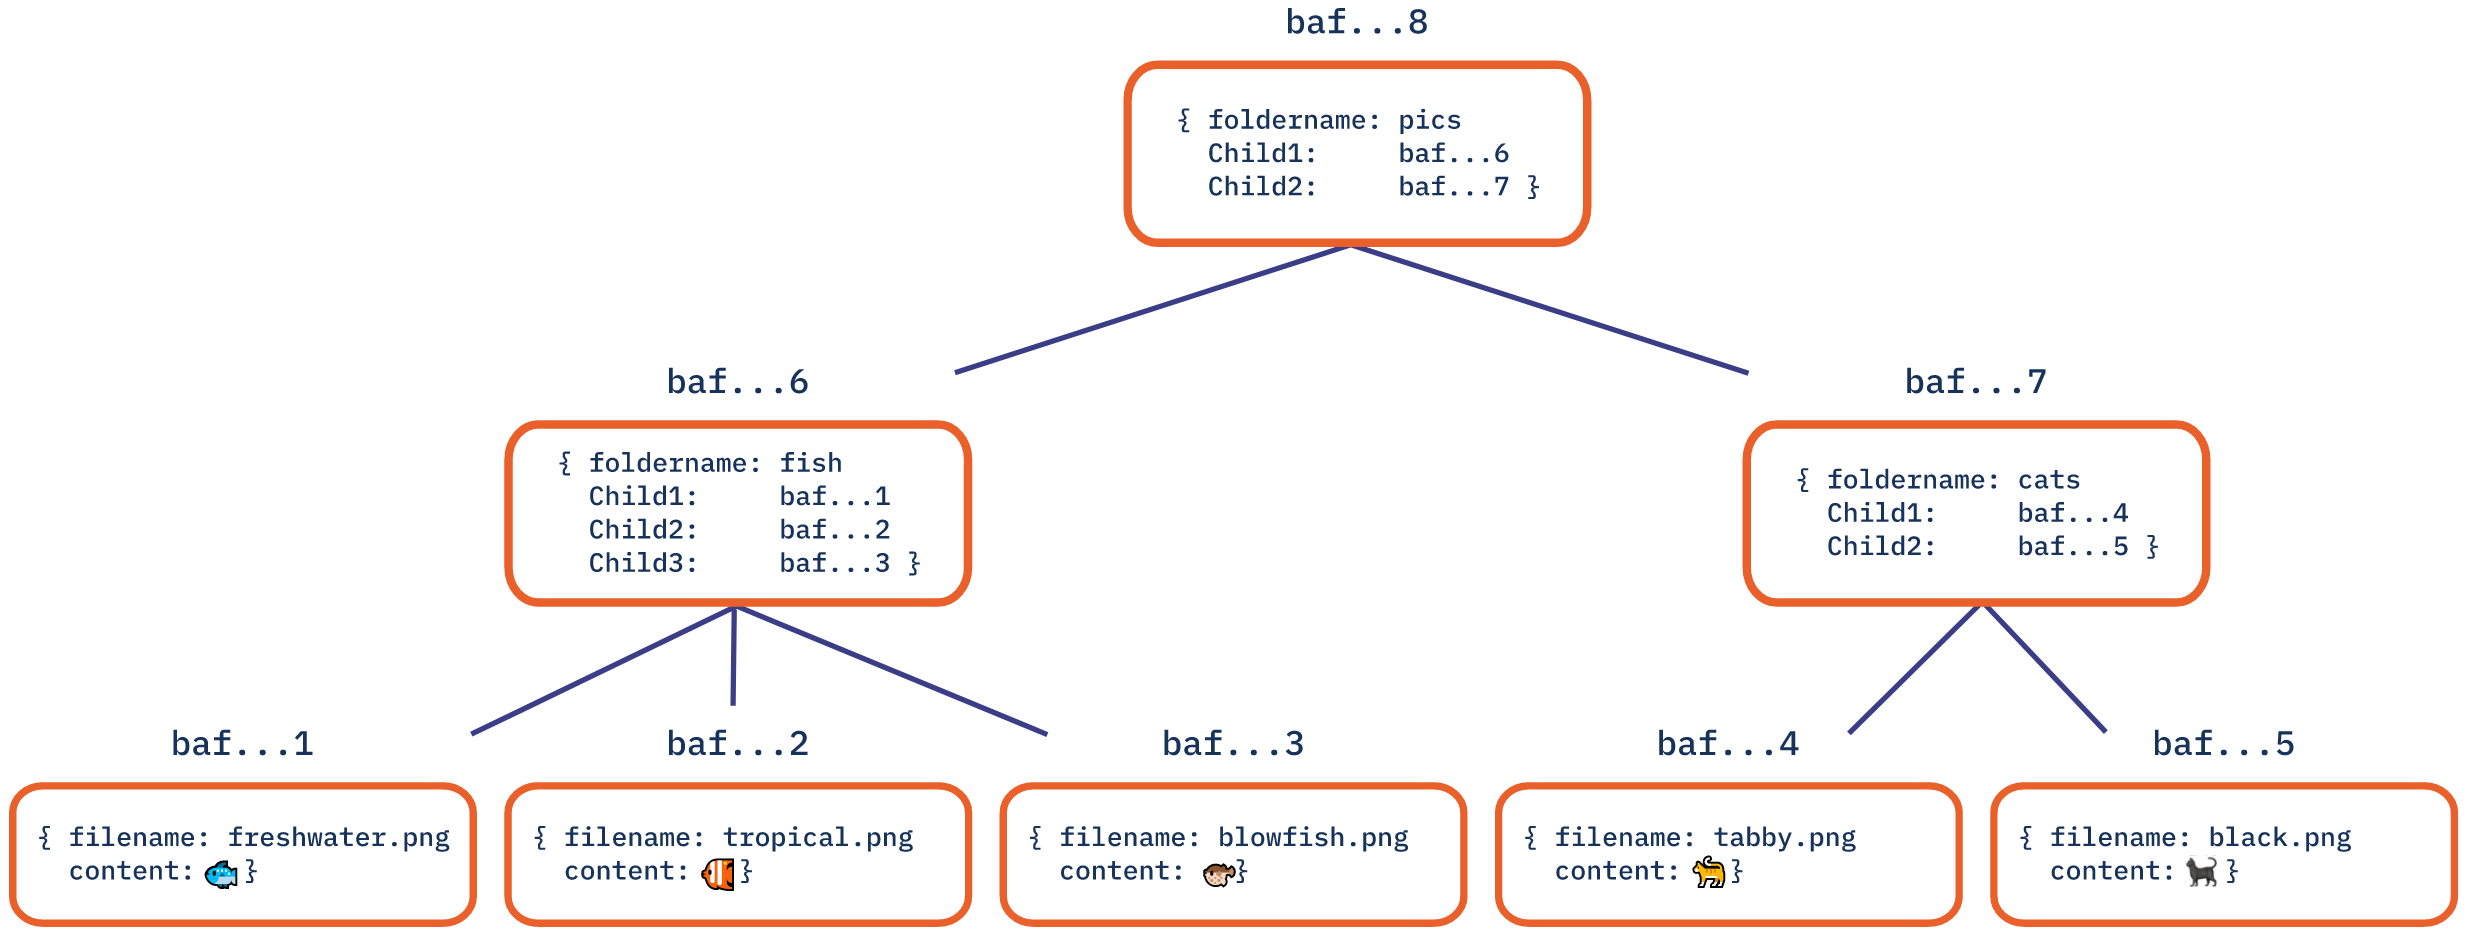
\includegraphics[width=.95\textwidth]{assets/figures/chapter-2/2.7.merkle-dag.png}
		\caption[Παράδειγμα Merkle DAG]{Παράδειγμα Merkle DAG\footnotemark}
	\end{enumitemcenteredfigure}
	\footnotetext{\url{https://proto.school/merkle-dags/}}

	Στο παραπάνω Merkle DAG τα baf...i αποτελούν τα CID των αρχείων και των φακέλων. Το δένδρο δημιουργείται από κάτω προς τα πάνω, υπολογίζοντας κάθε φορά τα κατάλληλα hashes/CIDs. Σε περίπτωση που το περιεχόμενο ενός κόμβου αλλάξει, τότε αλλάζει τόσο το CID του, όσο και τα CIDs όλων των προγόνων του.
	\item \textbf{Ανακάλυψη περιεχομένου μέσω κατανεμημένων πινάκων κατακερματισμού (\textenglish{Distributed Hash Tables ή DHTs})}. Ο DHT είναι ένα κατανεμημένο σύστημα για την αντιστοίχιση κλειδιών σε τιμές. Στο IPFS αποτελεί το θεμελιώδες συστατικό του συστήματος δρομολόγησης περιεχομένου και λειτουργεί ως διασταύρωση μεταξύ καταλόγου και συστήματος πλοήγησης. Πρακτικά πρόκειται για ένα πίνακα που αποθηκεύει ποιος έχει ποια δεδομένα και, μέσω του οποίου, ο χρήστης βρίσκει τον peer που έχει αποθηκευμένο το επιθυμητό περιεχόμενο.
\end{itemize}

Κάτι που θα πρέπει να σημειωθεί είναι πως, σαν προεπιλογή, οι IPFS κόμβοι αντιμετωπίζουν τα αποθηκευμένα δεδομένα ως προσωρινή μνήμη (cache), πράγμα που σημαίνει ότι δεν υπάρχει καμία εγγύηση ότι εκείνα θα συνεχίσουν να παραμένουν αποθηκευμένα σε αυτούς. Για την αποφυγή της διαγραφής τους από τον garbage collector, τα δεδομένα θα πρέπει να σημανθούν ως σημαντικά, μέσω του "καρφιτσώματος" (pinning). Έτσι, για την ομαλή λειτουργία π.χ. μίας DApp που βασίζεται στο IPFS, θα πρέπει το περιεχόμενό της να είναι pinned από αρκετούς peers και/ή να γίνεται χρήση κάποιου pinning service, ώστε να εξασφαλίζεται διαθεσιμότητά του.

Βασικό πλεονέκτημα του IPFS είναι ότι ο αποκεντρωτικός του χαρακτήρας δίνει τη δυνατότητα να παρέχεται το περιεχόμενο από πολλούς κόμβους, οι οποίοι βρίσκονται σε διαφορετικές τοποθεσίες και δεν υπάγονται σε κάποια συγκεκριμένη κεντρική αρχή. Με αυτόν τον τρόπο, τα δεδομένα είναι πιο ανθεκτικά τόσο από άποψη διαθεσιμότητας (αν ένας κόμβος αποσυνδεθεί, θα υπάρχει κάποιος άλλος), όσο και από άποψη αντοχής στη λογοκρισία. Μπορεί, επίσης, να ανακτώνται γρηγορότερα, εφόσον τα διαθέτουν κάποιοι κοντινοί peers, πράγμα ιδιαίτερα πολύτιμο για κοινότητες που είναι καλά δικτυωμένες τοπικά αλλά δεν έχουν καλή σύνδεση με το ευρύτερο διαδίκτυο.